%---------- Inleiding ---------------------------------------------------------

\section{Introductie}%
\label{sec:introductie}

Waarover zal je bachelorproef gaan? Introduceer het thema en zorg dat volgende zaken zeker duidelijk aanwezig zijn:

\begin{itemize}
  \item kaderen thema
  \item de doelgroep
  \item de probleemstelling en (centrale) onderzoeksvraag
  \item de onderzoeksdoelstelling
\end{itemize}

Denk er aan: een typische bachelorproef is \textit{toegepast onderzoek}, wat betekent dat je start vanuit een concrete probleemsituatie in bedrijfscontext, een \textbf{casus}. Het is belangrijk om je onderwerp goed af te bakenen: je gaat voor die \textit{ene specifieke probleemsituatie} op zoek naar een goede oplossing, op basis van de huidige kennis in het vakgebied.

De doelgroep moet ook concreet en duidelijk zijn, dus geen algemene of vaag gedefinieerde groepen zoals \emph{bedrijven}, \emph{developers}, \emph{Vlamingen}, enz. Je richt je in elk geval op it-professionals, een bachelorproef is geen populariserende tekst. Eén specifiek bedrijf (die te maken hebben met een concrete probleemsituatie) is dus beter dan \emph{bedrijven} in het algemeen.

Formuleer duidelijk de onderzoeksvraag! De begeleiders lezen nog steeds te veel voorstellen waarin we geen onderzoeksvraag terugvinden.

Schrijf ook iets over de doelstelling. Wat zie je als het concrete eindresultaat van je onderzoek, naast de uitgeschreven scriptie? Is het een proof-of-concept, een rapport met aanbevelingen, \ldots Met welk eindresultaat kan je je bachelorproef als een succes beschouwen?

%---------- Stand van zaken ---------------------------------------------------

\section{State-of-the-art}%
\label{sec:state-of-the-art}

Hier beschrijf je de \emph{state-of-the-art} rondom je gekozen onderzoeksdomein, d.w.z.\ een inleidende, doorlopende tekst over het onderzoeksdomein van je bachelorproef. Je steunt daarbij heel sterk op de professionele \emph{vakliteratuur}, en niet zozeer op populariserende teksten voor een breed publiek. Wat is de huidige stand van zaken in dit domein, en wat zijn nog eventuele open vragen (die misschien de aanleiding waren tot je onderzoeksvraag!)?

Je mag de titel van deze sectie ook aanpassen (literatuurstudie, stand van zaken, enz.). Zijn er al gelijkaardige onderzoeken gevoerd? Wat concluderen ze? Wat is het verschil met jouw onderzoek?

Verwijs bij elke introductie van een term of bewering over het domein naar de vakliteratuur, bijvoorbeeld~\autocite{Hykes2013}! Denk zeker goed na welke werken je refereert en waarom.

Draag zorg voor correcte literatuurverwijzingen! Een bronvermelding hoort thuis \emph{binnen} de zin waar je je op die bron baseert, dus niet er buiten! Maak meteen een verwijzing als je gebruik maakt van een bron. Doe dit dus \emph{niet} aan het einde van een lange paragraaf. Baseer nooit teveel aansluitende tekst op eenzelfde bron.

Als je informatie over bronnen verzamelt in JabRef, zorg er dan voor dat alle nodige info aanwezig is om de bron terug te vinden (zoals uitvoerig besproken in de lessen Research Methods).

% Voor literatuurverwijzingen zijn er twee belangrijke commando's:
% \autocite{KEY} => (Auteur, jaartal) Gebruik dit als de naam van de auteur
%   geen onderdeel is van de zin.
% \textcite{KEY} => Auteur (jaartal)  Gebruik dit als de auteursnaam wel een
%   functie heeft in de zin (bv. ``Uit onderzoek door Doll & Hill (1954) bleek
%   ...'')

Je mag deze sectie nog verder onderverdelen in subsecties als dit de structuur van de tekst kan verduidelijken.

%---------- Methodologie ------------------------------------------------------
\section{Methodologie}%
\label{sec:methodologie}

In deze studie zal een onderzoek gebeuren de bijdrage van een configuratie inventaris van Linux-systemen, bij het initiele proces van incident response bij een cyberaanval. Het onderzoek zal bestaan uit vijf fasen, zoals weergegeven in figuur~\ref{fig:chart}.

De eerste fase, literatuurstudie, richt zich op een diepgaand literatuuronderzoek om de impact van cybersecurity-incidenten te vergelijken tussen bedrijven met en zonder een uitgebreide inventaris. Het resultaat omvat een literatuurstudie die niet alleen de impact belicht, maar ook eigenschappen van Linux-toestellen identificeert die relevant zijn voor de inventaris.

De tweede fase, risico-analyse, concentreert zich op een kritische evaluatie van de ge\"edentificeerde Linux-toesteleigenschappen binnen de inventaris. Via een diepgaande risico-analyse worden de impact van deze eigenschappen op het incidentresponseproces en hun bruikbaarheid geëvalueerd. De risico-analyse omvat tevens een beoordeling van mogelijke kosten, waaronder financiële, energetische en tijdsinvesteringen, om het inventarisatieproces te verwezenlijken. Het resultaat van deze fase is een lijst van eigenschappen die een positieve bijdrage leveren aan het incident response proces, en een lijst van eigenschappen die een negatieve impact hebben op het incident response proces. Deze lijsten zullen worden gebruikt in de volgende fase.

Tijdens de derde fase, Proof-of-Concept, staat de ontwikkeling van een Bash-script centraal, gekoppeld aan het opzetten van een Proof-of-Concept omgeving. Het Bash-script beoogt een inventaris op te stellen met de in fase 2 geselecteerde eigenschappen. Testen vinden plaats op twee verschillende machines - een Red Hat Enterprise Linux (RHEL) webserver en een Debian mariadb database server met RAID 5-configuratie, in een virtuele omgeving met behulp van Vagrant. Het resultaat van deze fase is een werkend Bash-script dat een inventaris van een Linux-toestel opstelt, en een Proof-of-Concept omgeving waarin het Bash-script wordt uitgevoerd op een geautomatiseerde manier.

Na het uitvoeren van het Proof-of-Concept worden de resultaten geanalyseerd, dat de basis zal vormen voor de conclusie, waarbij de focus ligt op de kwaliteit en bruikbaarheid van de inventaris. Beoordelingscriteria omvatten de volledigheid van de inventaris, de aanwezigheid van fouten en de impact op het incidentresponseproces. De conclusie biedt beknopt, maar helder inzicht in de bevindingen en antwoordt op de onderzoeksvraag.

De afsluitende fase richt zich op de voltooiing van de paper. Ontbrekende hoofdstukken worden aangevuld, en de tekst wordt nauwkeurig nagelezen. Het resultaat is een voltooide scriptie die voldoet aan alle vereiste normen en essenti\"ele hoofdstukken omvat.

\begin{figure}
    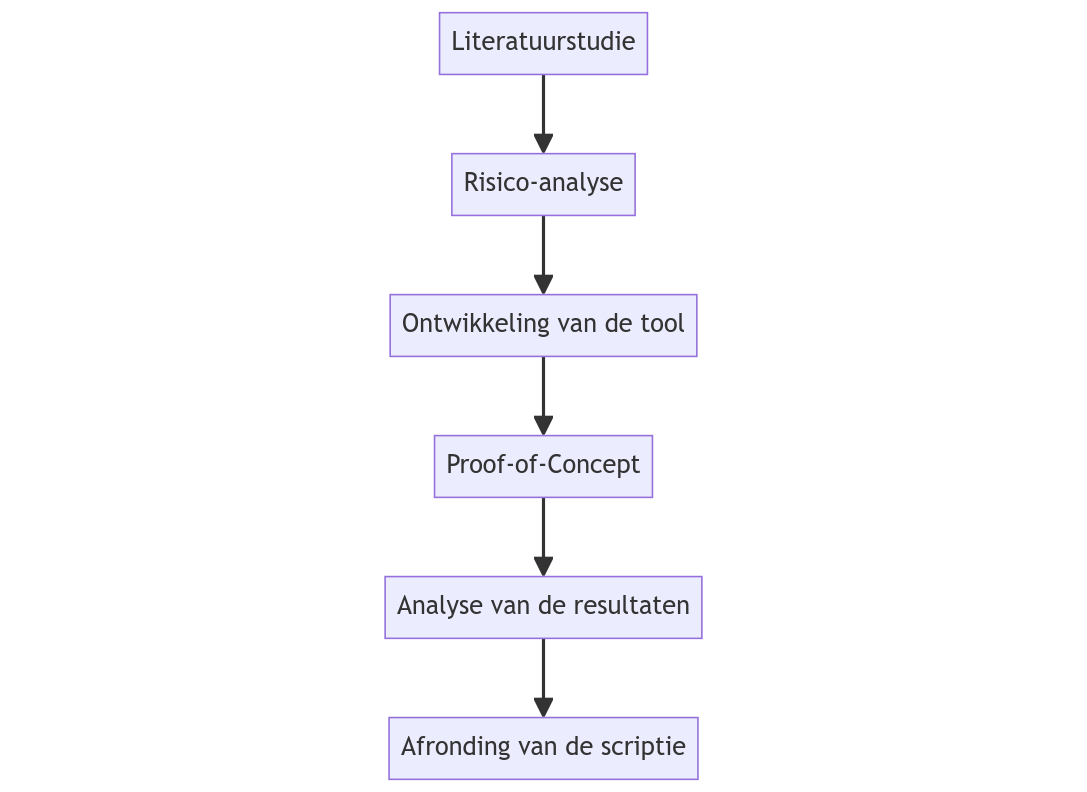
\includegraphics[width=.49\textwidth]
    {graphics/methodologie_flowchart.png}
    \caption{\label{fig:chart}Flowchart van de verschillende fasen in de methodologie}
\end{figure}

%---------- Verwachte resultaten ----------------------------------------------
\section{Verwacht resultaat, conclusie}%
\label{sec:verwachte_resultaten}

De verwachte resultaten van dit onderzoek omvatten een aanzienlijke bijdrage aan het incident response proces bij cyberaanvallen. Door het automatisch genereren van een gedetailleerde inventaris van Linux-systemen kunnen organisaties strategischer redeneren over de kritieke en minder kritieke systemen. Hierdoor wordt de efficiëntie van incident response verhoogd, met een gerichte aanpak op basis van de verzamelde gegevens.

Het inventaris automatiseren draagt bij aan het actueel houden van de inventaris, waardoor deze direct beschikbaar is wanneer nodig. Dit komt vooral van pas bij het identificeren van de meest kritische systemen tijdens een cybersecurity-incident, waardoor de reactietijd wordt verkort en de schade beperkt.

Hoewel grotere bedrijven vaak hun volledige stack automatiseren met tools zoals Ansible, kan de ontwikkelde methode met name waardevol zijn voor kleine en middelgrote ondernemingen. KMO's hebben doorgaans beperktere middelen en kunnen niet altijd profiteren van uitgebreide automatiseringsoplossingen. Daarom kan het geautomatiseerde inventarisatieproces een cruciale rol spelen in het versterken van de cybersecuritymaatregelen van KMO's, waar handmatige inventarisatie vaak tijdrovend en foutgevoelig is.
